% !TeX root = ../main.tex
% Add the above to each chapter to make compiling the PDF easier in some editors.

\chapter{Experimental Results}\label{chapter:results}

{\color{red} SOME INTRO SUMMARIZING THE FINDINGS IN BULLET POINTS}

We describe the complete experimental setups in Appendix \ref{appendix:experimental_setups}.

\section{Euclidean Flow Between Two Gaussians} \label{sec:gaussian_flow}

\begin{figure}[h!]
    \centering
    \begin{subfigure}{0.47\linewidth}
        \centering
        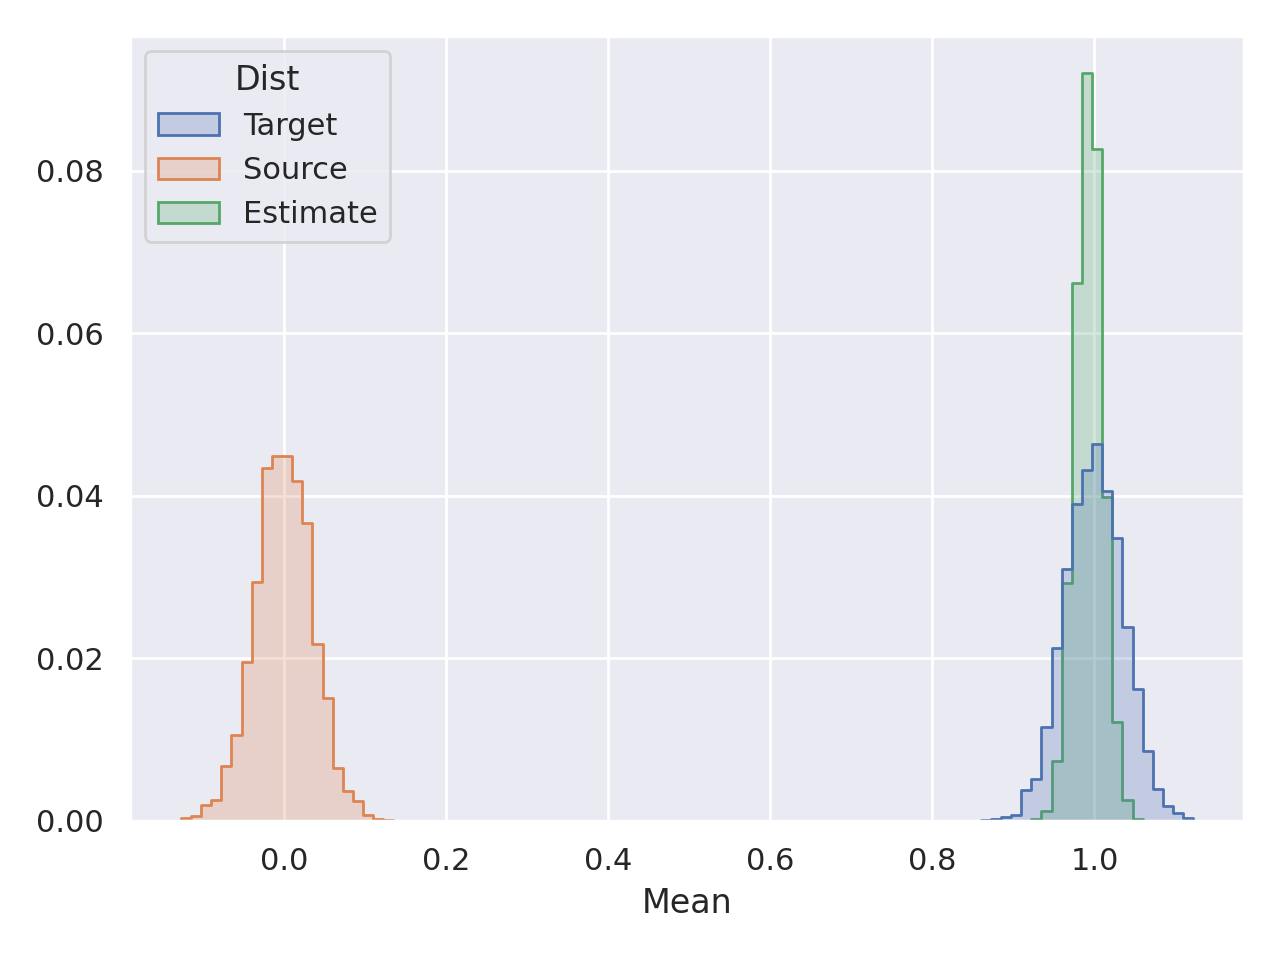
\includegraphics[width=\linewidth]{figures/gaussian/0.png}
        \caption{Deterministic sampling $(\varepsilon = 0)$}
        \label{fig:gaussian_deterministic}
    \end{subfigure}
    \begin{subfigure}{0.47\linewidth}
        \centering
        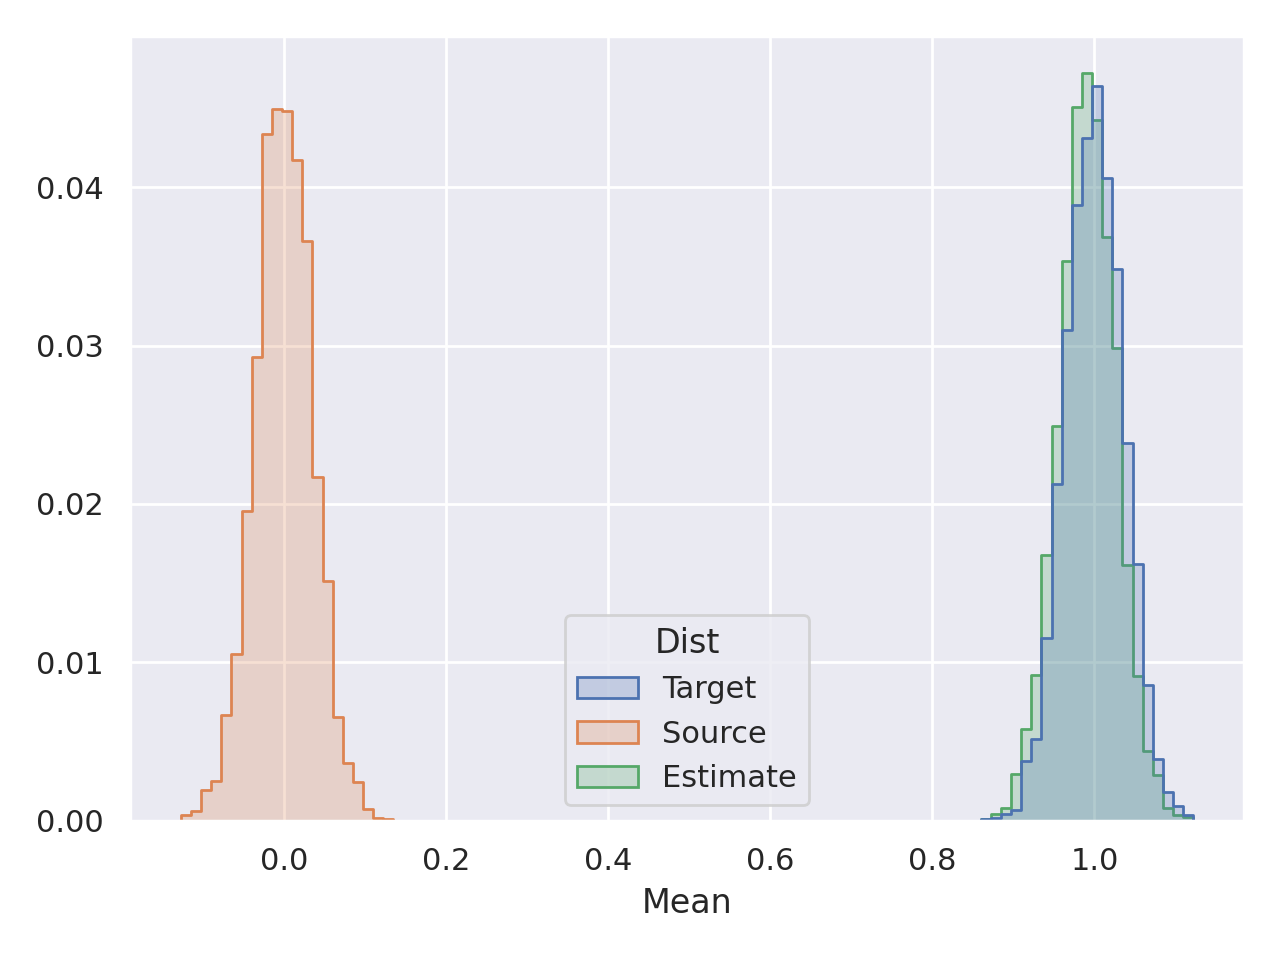
\includegraphics[width=\linewidth]{figures/gaussian/0.05.png}
        \caption{Stochastic sampling $(\varepsilon = 0.05)$}
        \label{fig:gaussian_stochastic}
    \end{subfigure}
    \caption{\label{fig:gaussian-results}\textbf{Histograms for the means of the weights generated by a Euclidean flow trained between two Gaussian distributions.} The flow fails to capture the variance in the target distribution with deterministic sampling, but this is corrected by stochastic sampling with $\varepsilon = 0.05$.} 
\end{figure}

To verify our approach of learning a flow model in weight-space, we begin our evaluation the toy task of learning a flow between two Gaussian distributions. The neural network is a small MLP with 30 input, two output dimensions, and two hidden layers of 16 neurons. We sample $X_0 \sim p_0 := \N(0, \mathbf{I})$ and $X_1 \sim p_1 := \N(1, \mathbf{I})$, and train our Euclidean flow to map $p_0$ to $p_1$ with independent coupling $q(x_0, x_1) = p_0(x_0)p_1(x_1)$. This is a relatively simpler task than learning over actual weights since each weight is sampled independently. 

Figure \ref{fig:gaussian-results} shows histograms of the means of the weights sampled from the flow with 100 Euler steps, and either deterministic or stochastic $(\varepsilon=0.05)$ sampling. Independent of the sampling method used, the flow covers the high-density center of the target distribution well, but the weights sampled deterministically fail to capture the variance in the target distribution. Stochastic sampling however appears to correct for this over-saturation and leads to more diverse samples. Overall, these results validates the feasability of learning a flow model in weight-space using graph neural networks, and we move on to tasks involving actual learned weights. 

\begin{figure}[t!]
    \centering
    \begin{subfigure}{0.47\linewidth}
        \centering
        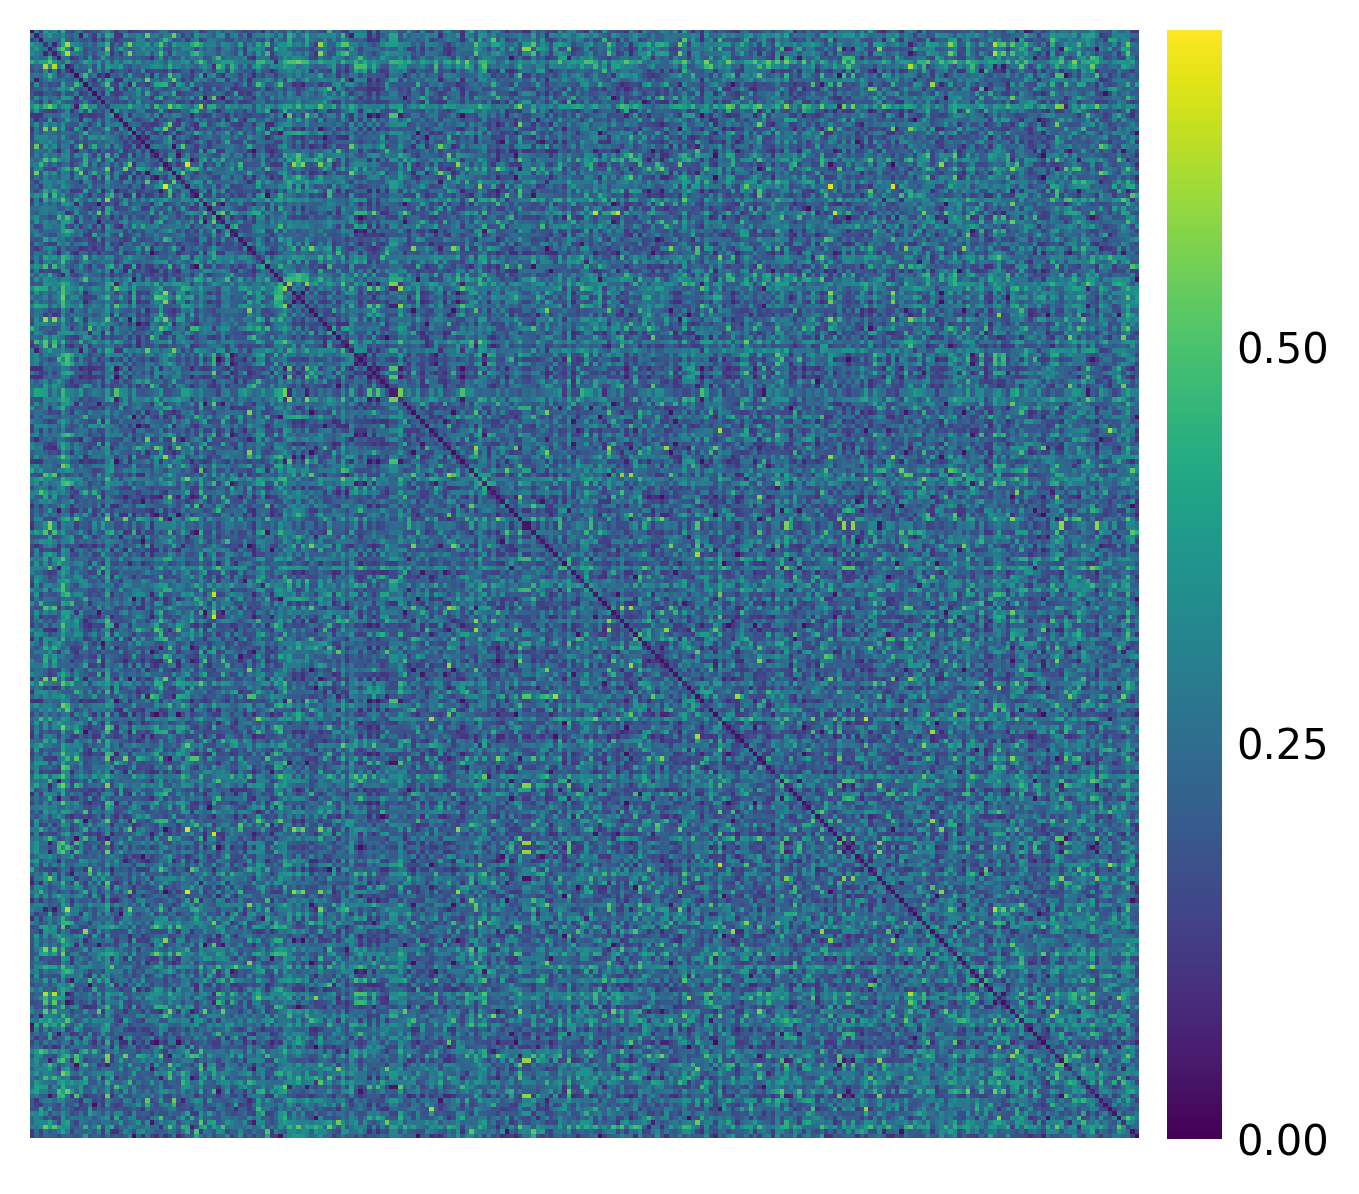
\includegraphics[width=\linewidth]{figures/uci_17/uci_17_unaligned.png}
        \caption{Unaligned (0.244 ± 0.009)}
        \label{fig:uci_unaligned}
    \end{subfigure}
    \begin{subfigure}{0.47\linewidth}
        \centering
        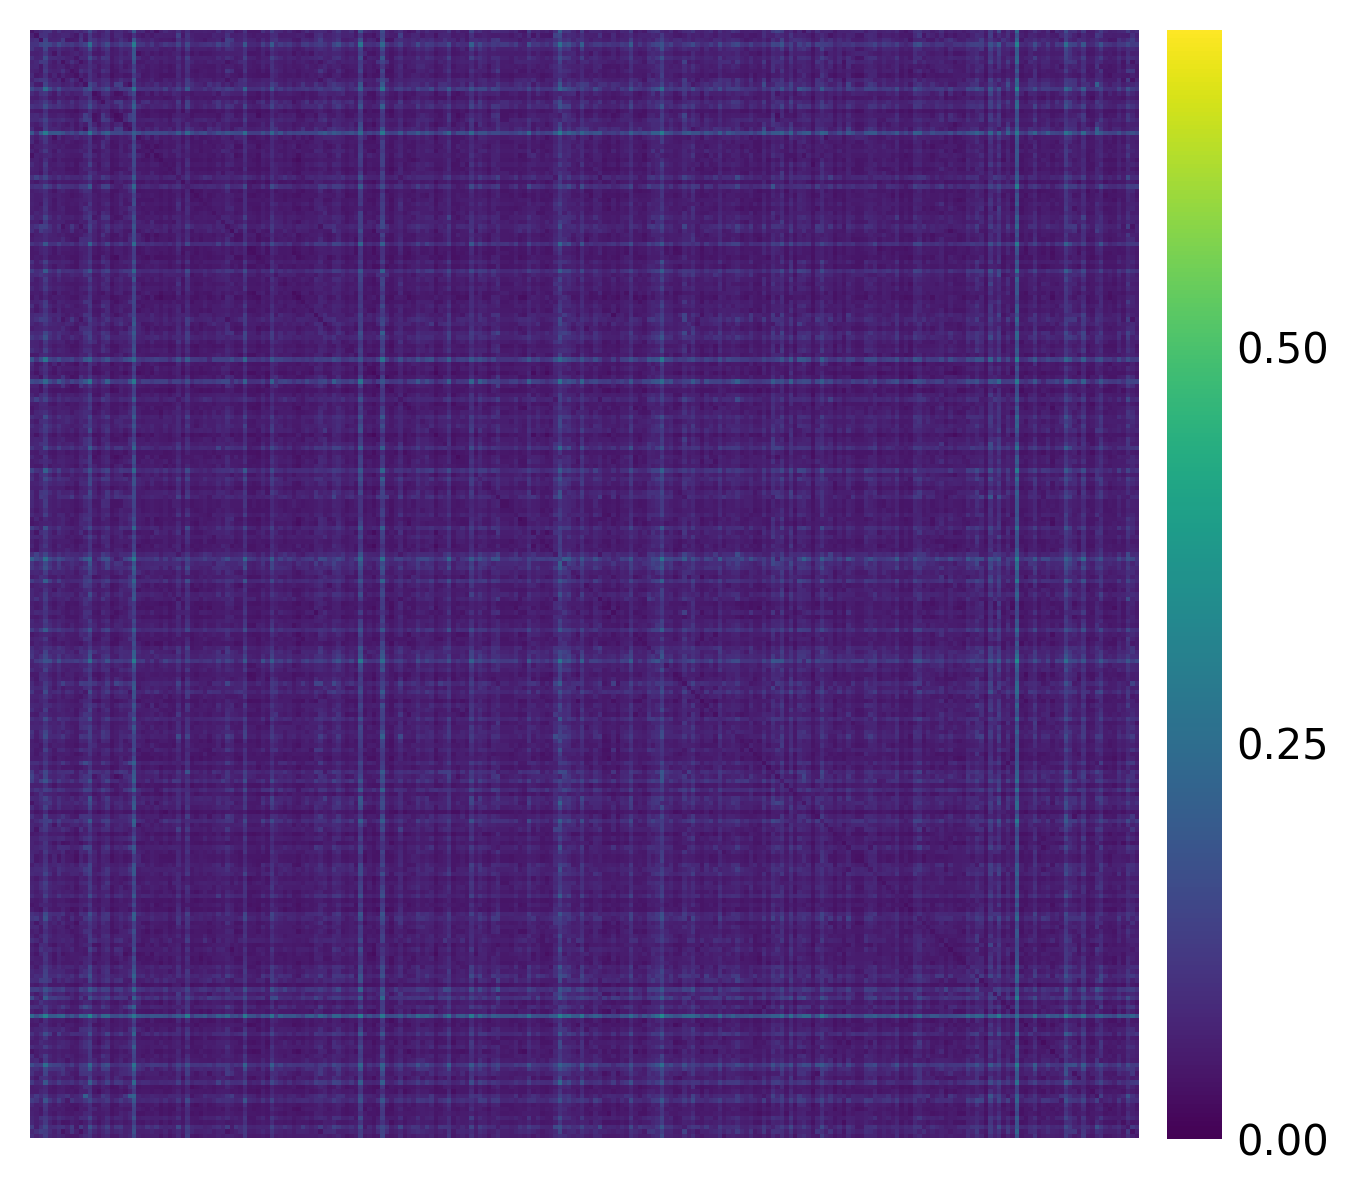
\includegraphics[width=\linewidth]{figures/uci_17/uci_17_aligned.png}
        \caption{Aligned (0.070 ± 0.001)}
        \label{fig:uci_aligned}
    \end{subfigure}
    \caption{\label{fig:uci_alignment}\textbf{Loss barriers for 250 weights across different optimization trajectories} (mean and standard deviations in parentheses) on the UCI Wisconsin Breast Cancer Diagnostics dataset. Aligning all weights to a single reference significantly reduces the loss barriers between the weights. } 
\end{figure}

\section{Classification with a Small Model}


\begin{table}[t!]
    \centering
    \begin{tabular}{lll}
        \toprule
        \textbf{Flow}  & \textbf{Accuracy} & \textbf{Loss} \\
        \midrule
        Euclidean                   & 0.998 ± 0.006     & 0.101 ± 0.05 \\ 
        Euclidean (aligned)         & 0.998 ± 0.006     & 0.070 ± 0.04 \\
        Euclidean (aligned + OT)    & 0.993 ± 0.010     & 0.053 ± 0.028 \\
        \midrule
        Normalized                  & 0.993 ± 0.009     & 0.027 ± 0.014 \\
        Normalized (aligned)        & 0.989 ± 0.011     & 0.030 ± 0.015 \\
        Normalized (aligned + OT)   & 0.988 ± 0.018	    & 0.044 ± 0.047 \\
        \midrule
        Geometric                   & 0.815 ± 0.279     & 0.525 ± 0.81 \\
        Geometric (aligned)         & 0.819 ± 0.277     & 0.551 ± 0.872 \\
        Geometric (aligned + OT)    & 0.812 ± 0.279 	& 0.530 ± 0.788 \\
        \midrule
        \textbf{Target}             & 0.992 ± 0.01      & 0.048 ± 0.032 \\
        \bottomrule
    \end{tabular}
    \caption{\label{tab:uci_class_table}\textbf{Test accuracy and loss ($\pm$ std) of the samples generated by flows with different design choices.} Euclidean and Normalized flows result in the most accurate weights, with Normalized flow generating lower-loss weights.}
\end{table}

After the toy Gaussian example, we move on to a relatively simple classification task to demonstrate that our flows can generate high-quality samples and compare the various design choices outlines in Chapter \ref{chapter:method}. The target model is an MLP with two hidden layers of 16 dimensions each and ReLU activations, on the binary classification task of the UCI Wisconsin Breast Cancer Diagnostic dataset \citep{streetNuclearFeatureExtraction1993}. We train all flows on the same dataset consisting of weights sampled from 100 independent trajectories optimized with Adam \citep{kingmaAdamMethodStochastic2017}. 

In addition to the availability of a large number of trained weights, this setup represents a preferable scenario in the sense that aligning all weights to a single reference eliminates the loss barriers between them to a large extent. Figure \ref{fig:uci_alignment} shows the pair-wise loss barriers (midpoint of the linear interpolation) before and after alignment for 250 randomly sampled weights from the set of Adam-optimized weights. The loss barriers are reduced considerably (from an average of 0.244 to 0.07) which supports the linear mode connectivity hypothesis for this setup. This should presumably make it easier to approximate the posterior distribution, as in the extreme case of zero-loss barriers between \textit{all} pairs of weights, the posterior would be convex. 

\textbf{Sample Quality.} Table \ref{tab:uci_class_table} compares the predictive quality of the samples generated by different flows. Although all flows can generate almost perfectly accurate samples, the Euclidean flow results in the highest average accuracy, followed by the Normalized flow. Although the accuracy of the samples generated by the Geometric flow are also within one standard deviation of the other two flows, they vary more significantly in quality. For this setup in particular, aligning the weights before training or training the flow with mini-batch optimal couplings do not provide a significant benefit, although that might be due to this being a relatively easy classification task. 

\begin{figure}[t!]
    \centering
    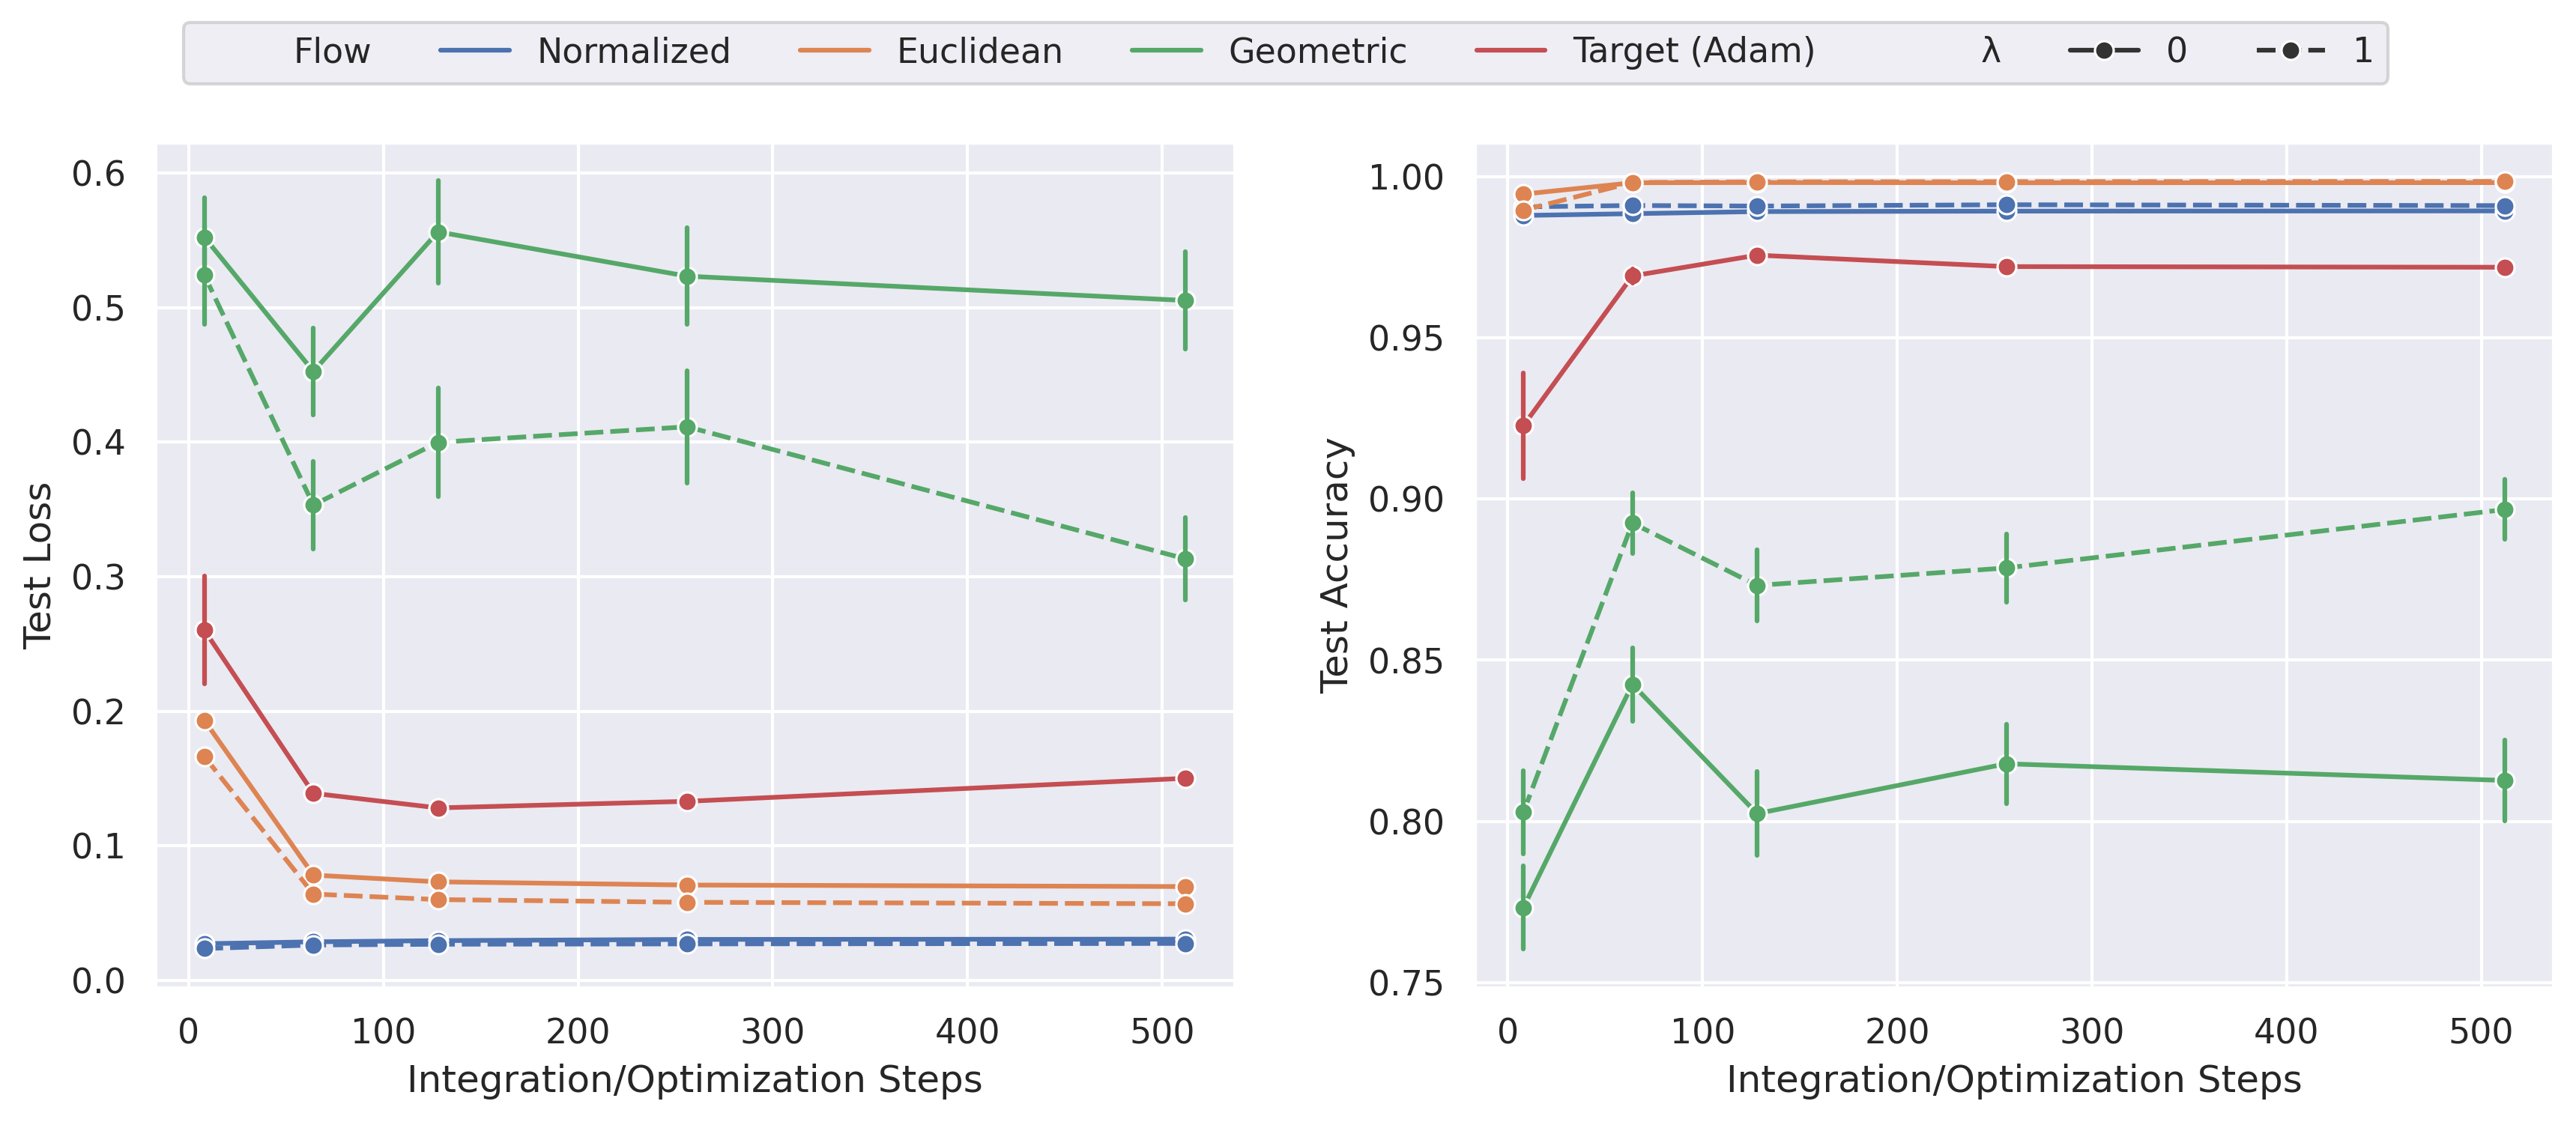
\includegraphics[width=\linewidth]{figures/uci_17/uci_17_steps_both.png}
    \caption{\label{fig:uci_steps}\textbf{Comparing the quality of the generated weights with Adam-optimized weights.} Weights generated by the Euclidean and Normalized flows have higher accuracy and lower loss than Adam-optimized weights, while the Geometric flow generated less accurate weights. Guidance during sampling improves sample quality.} 
\end{figure}

\textbf{Number of Integration Steps \& Guidance.} Figure \ref{fig:uci_steps} displays how the predictive performance of generated weights changes with the number of Euler steps performed to integrate the ODE. Most importantly, both the Euclidean and Normalized flows can sample weights with comparable loss and accuracy to those of Adam-optimized weights, in as low as 8 Euler steps. In particular, performing more Euler steps does not lead to a significant improvement in sample quality for the Normalized flow, indicating that it has learned straighter paths than an Euclidean flow. Guiding the sampling with gradients from the original task also improves the quality of generated samples. This improvement appears most significantly for the Geometric flow, likely due to the lower quality of its no-guidance samples. 



